\chapter{Introduction}
\label{chap:intro}

The use of high performance computers for  research in the Faculty of Engineering  and Applied Science has increased, because of increase in research tasks, such as testing new operating systems. As researchers demand robust computers, these computers systems also need to be expanded to accommodate these large tasks. As we expand the systems, access and usage  becomes more complicated to manage. Therefore we are faced with issues of system management, system accessibility, and storage. These issues are the inability to provide  a proper record of each computer system and its usage, the inability to provide flexible user access to the computers, and also the problem of monitoring the number of computers that are reserved by users. As a result of these challenges it is necessary to develop software that solves these problems for the Faculty of Engineering and Applied Science. 


Clowder is a system designed to provide a Preboot Execution Environment (PXE) for testing new operating systems through a Network File System (NFS) sever. Others have worked on this system for several years, but there was more work yet to be done to improve its existing features and functionality. As an example, it takes manual command line statements to access  a computer in the cluster during research. Another reason for improvement is to provide flexible and dynamic user interface rather than the current manual, error-prone norm (SSH). Therefore the current state of Clowder is not flexible and convenient enough. So the main goal of this project is to develop software that addresses the issue of user accessibility, system management and automatic control protocol. Addressing all these issues will improve the performance of Clowder in speed, access and robustness, making it a complete software tool. 
	
	
We have accomplished this goal by using a design approach that augments a previously existing interface and database system. The database system is designed to store and keep record of the computer systems and user activities. The web interface enable users to have access to the Clowder system from different locations simultaneously via a web page, and also provides users with the system inventory and other user activities. This  software provides the ability to search for data in the inventory, and to add new computer systems to the cluster, and to modify their properties individually. Also it provides the ability to make reservations: to allow users to reserve a computer for a certain period of time, and to end reservations as well.    
	

As this software serves as a tool to manage the cluster of computers and user activities, it is important to know that  reservations made, computer details, network interface cards and disks are stored as data. So all the computer system installed in the cluster with their names, vendors, memory size, architecture, and microarchitecture is stored in the database. The same is applicable to the disks, network interface cards and any other devices that could be part of the cluster. Data is represented as variables in their various data types in the database scheme.  All this information stored in the database tables serves as input  data for the program. This database scheme allows user to add or update new machines installed in the cluster, and therefore provide data record for the inventory on the web interface. 

The web interface serves as a platform for users to interact with the system and overview other users' activities via a web page. This interface can also  partially replace the SSH-accessible command line prompt which was the previous user interface for Clowder system. This choice provides flexible access to and control of the system, by allowing users to log on to the system and make requests of the inventory at any time through the web server.
\autoref{Designofprogram} shows a general description of the Clowder system.

\begin{figure}[h]
  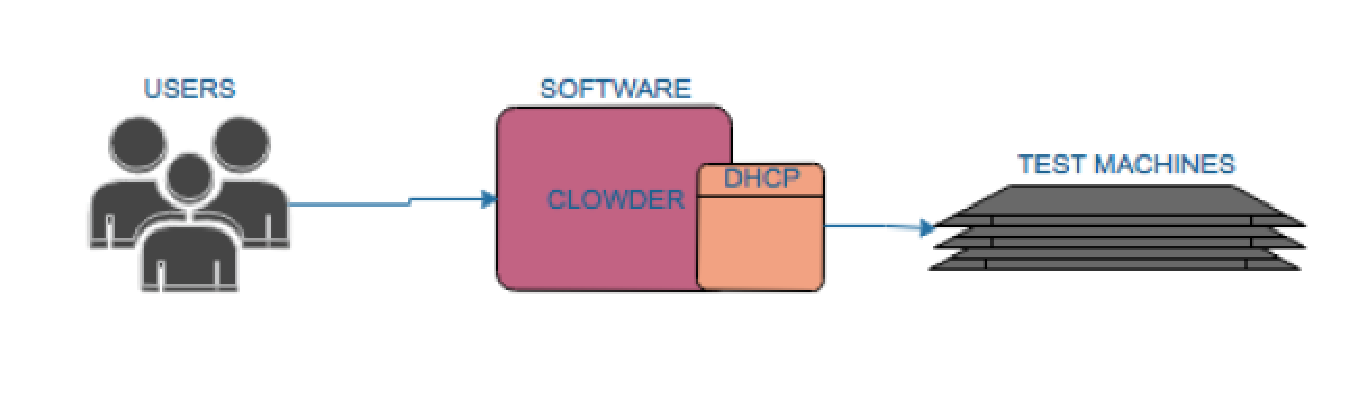
\includegraphics[width=\linewidth]{background.eps}
  \caption{A general design of the system}
  \label{Designofprogram}
\end{figure}
\pagebreak

This figure showcases the background concept of the Clowder as a full system. This concept is shown in detail in Fig 3.1, which explains the software functionality and data flow between the user interface and database. Following this chapter, we explain in more detail about the background of this system and other components that made up the design.

\section{Contribution}
I have contributed to this project to improve its existing interface and database functionality in other to have Clowder as complete software tool. My work includes the addition of required features to the interface such as; searching data from the system inventory, making reservation, checking for available machines, updating the system data, filtering and sorting the system inventory. These features were extended to the database improve its existing functionality. I have further explained this contributions in section \ref{Designstructure} and section \ref{Programstructure}.
